\chapter{Elliptic equations and the finite element method}


%\newcommand{\R}{\mathbb{R}}


\label{elliptic}
\section{Introduction}

As a starting point for the finite element method, let us
consider the mother problem of partial differential equations, 
the elliptic problem: Find the solution $u$ of the problem

\begin{eqnarray}
\label{elliptic}
-\nabla\cdot(k\nabla u)  &=& f \quad \textrm{in}\ \Omega,\\
\label{Dirichlet}
u&=& g \quad \textrm{on}\ \partial\Omega_D, \\
\label{Neumann}
\frac{\partial u}{\partial n}&=& h \quad \textrm{on}\ \partial\Omega_N . 
\end{eqnarray}
We include here both Dirichlet \eqref{Dirichlet} and Neumann \eqref{Neumann} boundary conditions
and assume $\partial \Omega = \partial \Omega_D \cup \partial \Omega_N$ 
and $\partial \Omega_D \cap \partial \Omega_N = \emptyset$.
 

Unusual concepts like weak or variational formulations, trial and test functions, Sobolev
spaces etc. show up in the finite element methods and many find them troublesome and strange. To motivate
these concepts we start with some "philosophical" considerations that lead to three observations which 
will be resolved by the finite element method. First, the above equation is 
the so-called strong formulation and its interpretation is (directly) that: \\ 
For every point $x \in \Omega$ the equation 
\begin{equation}
\label{strong:elliptic}
-\nabla\cdot(k(x) \nabla u(x))  = f(x),  
\end{equation}
should be valid. Hence, $u$, $f$ are functions and
if we assume that $f$ is a continuous function then $u$ is continuous with two derivatives that are also continuous.   
More formally, $f\in C(\Omega)$ directly leads to the requirement that $u\in C^2(\Omega)$. In general 
it is however well known, and we will meet many such solutions in this course, that $u \not \in C^2(\Omega)$ are also
solutions to \eqref{elliptic}. 



In this book, it will be sentral to compare differential operators with matrices in order to build
intuition. So, let us assume that  
\eqref{strong:elliptic} is somehow (ignoring the boundary conditions for now)  represented as a linear system, i.e.,  
\begin{equation}
\label{Aub}
A u = b .  
\end{equation}
This leads us to our second observation: In order to have a linear system with a well-defined solution we at least need the same number 
of equations and unknows, ie.  
$A$ is a $\R^{N\times N}$ matrix and $u$, $f$ are vectors in $\R^N$. How can we make numerical methods that ensure
the same number of equations and uknowns? Is it ensured by the definition in \eqref{strong:elliptic}.  
A direct comparison of \eqref{strong:elliptic} and \eqref{Aub} would for instance be to assume that $i$'th equation of $A u = b$ correspond to the point $x_i$ in
\eqref{strong:elliptic}. Hence, $\sum_j A_{ij} u_j = b_i$ corresponds
to $-\nabla\cdot(k(x_i) \nabla u(x_i))  = f(x_i)$.   
Then the number of equations (or number of rows in $A$) is $N$ and equals the number
of points in the domain.  Assuming for instance
that $\Omega$ is the unit square with $n$ internal points (as the boundary is currently ignored) in both the $x-$ and $y-$direction 
gives that $N=n^2$. With a slight abuse of notation\footnote{We avoid bold face notation for coordinates. }, we may then enumerate the points as
$x_i = (x_j, y_k)$ where $i = j(N-1) + k$ for $i,j \in (1, N)$.  
In order to get a non-singular matrix, the number of unknowns should
equal the number of equations. We do obtain $N$ uknowns if we assume that for every
point in the domain we have an unknown $u_k = u(x_i, y_j)$, $k=j+i(N-1)$ corresponding to  
the equations 
$-\nabla\cdot (k \nabla  u(x_i, y_j) = f(x_i, y_j)$. It is however not clear how to make sense of $u$ outside the points $(x_i, y_j)$.      
Furtermore, an obvious mathematical question is then to what extent we recover $ u \in C^2(\Omega), f \in C(\Omega)$ as $n$ tends to $\infty$
with this construction. In general, we will not recover the conditions set by the strong formulation, although a proper mathematical 
explanation of this is beyond the scope of this book. The reader is refered to \cite{evans2022partial} for a more detailed
explanation of the strong formulation. 


\begin{figure}
\begin{center}
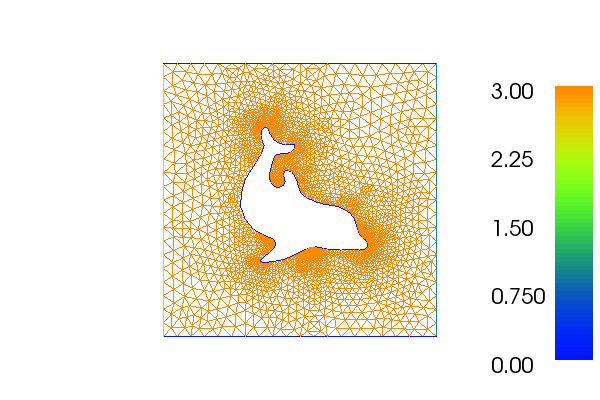
\includegraphics[width=0.75\textwidth]{chapters/elliptic/pics/dolfin_mesh.png}
\caption{An example mesh of a swimming dolphin.}
\label{fig:dolphin}
\end{center}
\end{figure}



For computational methods, we need to resort to finite resolution and this brings us to our third 
issue. In Figure \ref{fig:dolphin} we see triangulation of domain outside a swimming dolphin. We
can immediately see that it will be difficult to formulate a finite difference approach on this domain
as the nodal points does not form squares. Hence, a stencil like: 
\[
	\frac{u(x+h,y) + u(x,y+y) -4 u(x,y) + u(x-h,y) + u(x, y-h) }{h^2} (\approx \Delta u) 
\]
will not be able to exploit the triangulation. Furhermore, the stencil will cross $\partial \Omega$.   


\section{The finite element method in a nutshell}

The finite element method (FEM) resolves these three challenges by combining 1) the so-called weak formulations
to reduced the demands of differentiability of the solution with 2) a structured approach of integration
adjusted to the underlying meshes and 3) a polynomial approximation to achieve a versatile, practical, accurate
and efficient method. However, before we start with FEM, let us recap some fundamental results of calculus, 
Gauss-Green's lemma: 
\begin{equation}
\label{gaussgreen}
\int_\Omega 
-\nabla\cdot(k\nabla u) v \dx =  
\int_\Omega (k\nabla u) \cdot \nabla v \dx  - \int_{\partial \Omega} k\frac{\partial u} {\partial n} \ds 
\end{equation}

With this lemma in mind we transform equation \eqref{elliptic} into an integral integral equation by multiplying
\eqref{elliptic} with a test function $v$ before we integrate over the domain $\Omega$. Hence, 
we obtain  
\begin{equation}
\label{gaussgreen}
\int_\Omega -\nabla\cdot(k\nabla u) v \dx =  \int_\Omega f v \dx .  
\end{equation}
Here, $v$ plays the role the pointwise evaluation in the strong formulation. That is,
we may evaluate the above equation with respect to many different $v$'s. 
For instance, if the $v$'s are the Dirac delta functions corresponding to the points in $\Omega$, i.e.,  $v_k = \delta(x_i, y_j)$
then we obtain directly the strong formulation. This formulation is often called
the collocation method and is used e.g. for the Runge-Kutta method. However, it is 
seldom used for FEM because of the high demands on the differentiability on $u$. 

We arrive at the final weak formulation by two steps. First, we exploite the Gauss-Green's lemma. That is,  
\begin{eqnarray*}
\label{gaussgreen}
\int_\Omega f v \dx =   \int_\Omega -\nabla\cdot(k\nabla u) v \dx =  \\ 
\int_\Omega (k\nabla u) \cdot \nabla v \dx  - \int_{\partial \Omega} k\frac{\partial u} {\partial n} v \ds  .  
\end{eqnarray*}
Second, we apply the boundary conditions. That is, for the Dirichlet
condition \eqref{Dirichlet} we already know that $u=g$. Hence, $u$ is not an unknown at that part of the boundary.  Therefore, it is common 
to let $v=0$ at $\partial \Omega_D$. Furthermore, by inserting the Neumann condition, we obtain that  
\begin{eqnarray}
\int_{\partial \Omega} k\frac{\partial u} {\partial n} v ds =   
\int_{\partial \Omega_D} k\frac{\partial u} {\partial n} v ds +   \int_{\partial \Omega_N} k\frac{\partial u} {\partial n} v ds =   
\int_{\partial \Omega_D} k\frac{\partial u} {\partial n} 0 +   \int_{\partial \Omega_N} h v ds   
\end{eqnarray}
As such we arrive at the \emph{weak formulation} of the elliptic problem: 
Find $u$ such that 
\begin{equation}
\label{weakform}
\int_\Omega k \nabla u \cdot \nabla v dx = \int_\Omega f v dx + \int_{\Omega_N} h v ds, \quad \forall v  
\end{equation}
Here, we assume as mentioned that $u=g$ and $v=0$ on $\partial \Omega_D$. We will come back to what $\forall v$ means in a 
more precise sense later.  

\begin{figure}
\begin{center}
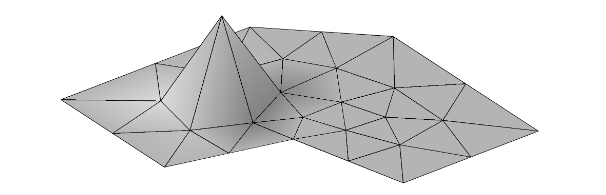
\includegraphics[width=0.75\textwidth]{chapters/elliptic/pics/fem.png}
\caption{One finite element basis function /pyramide function associated with a particular node.}
\label{fig:fembasis}
\end{center}
\end{figure}




The finite element method directly exploits the weak formulation. 
Let the trial and test functions be as follows:  
\begin{equation}
\label{trialtest}
u = \sum_j u_j N_j \quad \text{and} \quad v=N_i
\end{equation}
	. Here $\{N_i\}$ is a set of basis functions choosen somehow. 
There are many possibilities and one may target the basis function to the problem at hand. 
The simplest basis function is shown in 
Fig \ref{fig:fembasis}. Here, the basis function is chosen as linear functions / pyramides associated with the nodal points, 
so-called Lagrange element of first order.  
There are many, many different finite element functions to choose from and they have different properties. 
Lists of common and unusual elements available in FEniCS can be found in 
\cite{logg2012automated}. 

The FEM problem is obtained by inserting \eqref{trialtest} into the weak formulation, i.e.   
\[
\int_\Omega k \nabla \sum_j u_j N_j  \cdot \nabla N_i dx = \int_\Omega f N_i dx + \int_{\Omega_N} h N_i ds  \quad \forall j .    
\]
A simple rewrite: 
\[
\sum_j u_j  \int_\Omega k \nabla  N_j  \cdot \nabla N_i dx = \int_\Omega f N_i dx + \int_{\Omega_N} h N_i ds \quad \forall j.    
\]
Hence, with  
\begin{eqnarray*}
A_{ij} = \int_\Omega k \nabla  N_j  \cdot \nabla N_i dx, \\  
b_i = \int_\Omega f N_i dx + \int_{\Omega_N} h N_i ds 
\end{eqnarray*}
we arrive at the following linear system 
\[
A u = b 
\]

The following code solves the Poisson problem on the unit square
consisting of $32\times 32$ rectangles, where each rectangle is divided
in two and $f=1$, $g=0$ and $h=x$. Dirichlet conditions are set 
for $y=0$ and Neumann for the rest of $\partial \Omega$.  

\begin{python}
from dolfin import *

# Create mesh and define function space
mesh = UnitSquareMesh(32, 32)
V = FunctionSpace(mesh, "Lagrange", 1)

# Define Dirichlet boundary (x = 0 or x = 1)
def boundary(x): return x[0] < DOLFIN_EPS 

# Define boundary condition
u0 = Constant(0.0)
bc = DirichletBC(V, g, boundary)

# Define variational problem
u = TrialFunction(V)
v = TestFunction(V)
f = Constant(1)
g = Expression("x[0]")
a = inner(grad(u), grad(v))*dx
L = f*v*dx + h*v*ds

# Compute solution
u = Function(V)
solve(a == L, u, bc)

# Save solution in VTK format
file = File("poisson.pvd")
file << u
\end{python}

\section{Brief remark on the strange world of partial differential equations and their discretizations }

A fundamental property in both the theory of partial differential equations and numerical analysis is the
concept of well-posedness. In Hadamard's definition a problem is well-posed if a solution exists, is unique
and depends continuously on the input. Hence, if we have two inputs to our problem, $b_1$ and $b_2$ 
then the difference between the solutions $u_1$ and $u_2$ should be bounded by the differences
between $b_1$ and $b_2$. In terms of linear algebra, we directly obtain well-posedness if
$A$ is a non-singular matrix. That we directly have 
\[
\|A(u_1 - u_2) \| = \|b_1 - b_2\|     
\]
and 
\[
\|(u_1 - u_2) \| = \|A^{-1}b_1 - b_2\| \le  \|A^{-1}\| \|b_1 - b_2\|     
\]
which we directly can explore to obtain bounds. Neither of these observations are however
very useful. 
For instance, an intuitive estimate like  
\[
\|(u_1 - u_2) \|_\infty = \|(-\Delta)^{-1} \|_\infty \|f_1 - f_2\|_\infty     
\]
requires non-obvious regularity requirements. Here, 
$\|f \|_\infty = \sup_x |f(x)|$\footnote{Note that $\sup$ is an 
extension of $\max$ for infinite dimentional sets. In particular, $\sup=max$ for finite dimentional sets.}  

Instead, it is useful to consider the square roots for matrices and operators. 
We will make it more precise later, but let us assume 
that we have a concept of 
$A^{1/2}$ and $A^{-1/2}$. The, as we will see,  the notion 
\[
\|A^{1/2}(u_1 - u_2) \| = \|A^{-1/2}b_1 - b_2\|     
\]
is extraordinary useful and gives precise estimates in a wide range of situations.  
We remark that $\Delta=\nabla\cdot\nabla$ and as such $\nabla$ can be interpreted
as some kind of square root of $\Delta$. There are however some difficulties that
arise with this notion. Let us consider the problem in 1D, using FDM. The stencil 
is then 
\[
- u_{xx} \approx A u =  \frac{-u_{i+1} + 2 u_{i+1}  -u_{i-1}}{h^2}, 
\]  
where $u_i= u(x_i)$ and $x_i = ih, \ i=0,\ldots, N$. 
For a mesh with two internal degrees of freedom, the corresponding matrix 
is 
\[
A = 
\frac{1}{h^2}\begin{pmatrix}
2 & -1 \\ -1 & 2 
\end{pmatrix}
\]
Let $B$ 
\[
B u = 
\frac{1}{h}\begin{pmatrix}
1 & -1 & 0  \\ 0 & 1 & -1  
\end{pmatrix}
\]
Obviously,  
\[
A = B^T B 
\]
However, $B$ is not unique. Furthermore, it is a rectangular matrix that makes
it difficult to invert it. In particular, it has a one-dimentional kernel
consisting of the constant vector $c (1,1,1)^T$, where $c\in \R$. Likewise
in the continuous setting $\nabla$ has a kernel of constant functions.  
However, and withough any mathematical rigour, 
the correct and actually quite practical 
variant of the above estimate is    
\[
\|\nabla (u_1 - u_2) \| = \|\nabla^{-1}(f_1 - f_2)\|     
\]
We do however need to make sense of the 
$\nabla^{-1}$. For now it is enough to think of it as some form of antiderivative. 
Here, for instance $u_1, f_1$ may be the actual continuous solution and input data whereas the 
$u_2, f_2$ are the numerical solution and input data. 

\section{Further reading}
There are several execellent and highly recommended books on the finite element method~\cite{braess2007finite, brenner2008mathematical}. 


\section{Exercises}

\begin{exercise}
Consider the problem $-u''(x) = x^2$ on the unit interval with $u(0) = u(1) = 0$.  
Let $u=\sum_{k=1}^{10} u_k \sin(\pi k x )$ and $v=\sin(\pi l x)$ for $l=1, \ldots 10$
and solve \eqref{weakform}. What is the error in $L_2$ and $\L_\infty$.  
\end{exercise}

\begin{exercise}
Consider the same problem as in the previous exercise, but using Bernstein polynomials. 
That is, the basis for the Bernstein polynomial of order 10 on the unit interval is $B_k(x)=x^k(1-x)^{10-k}$ for $k=0, \ldots, 10$.  
Let $u=\sum_{k=0}^{10} u_k B_k(x )$ and $v=B_l(x)$ for $0=1, \ldots 10$
and solve \eqref{weakform}. What is the error in $L_2$ and $\L_\infty$.  
\end{exercise}

\begin{exercise}
Consider the same problem as in the previous exercise, but with  
$-u''(x) = sin(k \pi x)$ for $k=1$ and $k=10$.  
\end{exercise}

\begin{exercise}
Consider the same problem as in the previous exercise, but
with the finite element method in for example FEniCS, using Lagrange 
method of order 1, 2 and 3. 

\end{exercise}











